\documentclass[12pt,preprint]{aastex}

% has to be before amssymb it seems
\usepackage{color,hyperref}
\definecolor{linkcolor}{rgb}{0,0,0.5}
\hypersetup{colorlinks=true,linkcolor=linkcolor,citecolor=linkcolor,
            filecolor=linkcolor,urlcolor=linkcolor}

\usepackage{url}
\usepackage{algorithmic,algorithm}
\usepackage{multirow}

\usepackage{listings}
\definecolor{lbcolor}{rgb}{0.9,0.9,0.9}
\lstset{language=Python,
        basicstyle=\footnotesize\ttfamily,
        showspaces=false,
        showstringspaces=false,
        tabsize=2,
        breaklines=false,
        breakatwhitespace=true,
        identifierstyle=\ttfamily,
        keywordstyle=\bfseries\color[rgb]{0.133,0.545,0.133},
        commentstyle=\color[rgb]{0.133,0.545,0.133},
        stringstyle=\color[rgb]{0.627,0.126,0.941},
    }

\usepackage{amssymb,amsmath}

\newcommand{\project}[1]{{\sffamily #1}}
\newcommand{\Python}{\project{Python}}
\newcommand{\numpy}{\project{numpy}}
\newcommand{\bart}{\project{Bart}}
\newcommand{\emcee}{\project{emcee}}
\newcommand{\kepler}{\project{Kepler}}
\newcommand{\license}{MIT License}

\newcommand{\paper}{\emph{Article}}

\newcommand{\foreign}[1]{\emph{#1}}
\newcommand{\etal}{\foreign{et\,al.}}
\newcommand{\etc}{\foreign{etc.}}

\newcommand{\Fig}[1]{Figure~\ref{fig:#1}}
\newcommand{\fig}[1]{\Fig{#1}}
\newcommand{\figlabel}[1]{\label{fig:#1}}
\newcommand{\Tab}[1]{Table~\ref{tab:#1}}
\newcommand{\tab}[1]{\Tab{#1}}
\newcommand{\tablabel}[1]{\label{tab:#1}}
\newcommand{\Eq}[1]{Equation~(\ref{eq:#1})}
\newcommand{\eq}[1]{\Eq{#1}}
\newcommand{\eqlabel}[1]{\label{eq:#1}}
\newcommand{\Sect}[1]{Section~\ref{sect:#1}}
\newcommand{\sect}[1]{\Sect{#1}}
\newcommand{\App}[1]{Appendix~\ref{sect:#1}}
\newcommand{\app}[1]{\App{#1}}
\newcommand{\sectlabel}[1]{\label{sect:#1}}
\newcommand{\Algo}[1]{Algorithm~\ref{algo:#1}}
\newcommand{\algo}[1]{\Algo{#1}}
\newcommand{\algolabel}[1]{\label{algo:#1}}

% math symbols
\newcommand{\dd}{\ensuremath{\,\mathrm{d}}}
\newcommand{\bvec}[1]{\ensuremath{\boldsymbol{#1}}}
\newcommand{\unit}[1]{\ensuremath{\mathrm{#1}}}
\newcommand{\normal}[1]{\ensuremath{\mathcal{N}(#1)}}

\newcommand{\obs}[1]{\ensuremath{\overline{#1}}}

% abstract parameters
\newcommand{\hyperhyper}{\ensuremath{\lambda}}
\newcommand{\hyper}{\ensuremath{\theta}}
\newcommand{\local}{\ensuremath{w}}
\newcommand{\data}{\ensuremath{x}}

% hierarchical parameters
\newcommand{\rpop}{\ensuremath{\alpha}}
\newcommand{\Rpop}{\ensuremath{\beta}}
\newcommand{\selection}{\ensuremath{\delta}}

% PGM parameters
\newcommand{\rp}{\ensuremath{r}}
\newcommand{\ror}{\ensuremath{z}}
\newcommand{\rorobs}{\obs{\ror}}
\newcommand{\Rs}{\ensuremath{R}}
\newcommand{\Rsobs}{\obs{\Rs}}
\newcommand{\sigmasobs}{\obs{\sigma}}
\newcommand{\sn}{\ensuremath{\Sigma}}
\newcommand{\isobs}{\obs{q}}

% Selection parameters
\newcommand{\Pmax}{\ensuremath{P_\mathrm{max}}}
\newcommand{\selectwidth}{\ensuremath{\Delta}}
\newcommand{\snmin}{\ensuremath{\Sigma_\mathrm{min}}}


\begin{document}

\title{%
Inferring the exoplanet radius distribution from a noisy, incomplete catalog
}

\newcommand{\nyu}{2}
\newcommand{\mpia}{3}
\author{%
    Daniel~Foreman-Mackey\altaffilmark{1,\nyu},
    David~W.~Hogg\altaffilmark{\nyu,\mpia},
    \etal
}
\altaffiltext{1}{To whom correspondence should be addressed:
                        \url{danfm@nyu.edu}}
\altaffiltext{\nyu}{Center for Cosmology and Particle Physics,
                        Department of Physics, New York University,
                        4 Washington Place, New York, NY, 10003, USA}
\altaffiltext{\mpia}{Max-Planck-Institut f\"ur Astronomie,
                        K\"onigstuhl 17, D-69117 Heidelberg, Germany}

\begin{abstract}
The catalog of \kepler\ Objects of Interest (KOI) is a list of putative periodic exoplanet transit signals
  discovered in the photometric data from the \kepler\ Satellite.
In principle this catalog contains a wealth of statistical information about the full population of exoplanets.
Here we construct a model of the population that explains the content of the catalog.
Our approach is novel in that
  it takes the form of a rigorous (if approximate) hierarchical Bayesian inference,
  it includes a parameterization of a non-trivial selection function (incompleteness),
  and we fully marginalize out all latent and nuisance parameters using sampling.
Because the model is properly hierarchical,
  it can be constrained by multiple data sources;
  we demonstrate this by adding the Solar System as a constraint,
  but extensions to radial velocity, direct detection, and astrometric surveys would also be straightforward.
Approximations abound:
  Simple parameterized forms are assumed for the multivariate distribution of exoplanet parameters,
  incompleteness is assumed to depend only on a scalar related to signal-to-noise,
  and the KOI catalog is assumed to be dominated by real (not false-positive) exoplanet signals.
We find XXX and YYY.
\end{abstract}

\keywords{% CUT THESE DOWN TO SIX
  astronomical~databases:~miscellaneous
  ---
  catalogs
  ---
  eclipses
  ---
  methods:~statistical
  ---
  planetary~systems
  ---
  planets~and~satellites:~detection
  ---
  planets~and~satellites:~fundamental~parameters
  ---
  stars:~statistics
  ---
  surveys
}

\section{Introduction}

Obvious righteousness of following the laws of probability theory.

Moderate wrongness (but sensibleness) of histogramming maximum-likelihood estimates.
Even inverse-completeness weighted.

Terrible wrongness of co-adding posteriors or smoothing a histogram of estimates with the uncertainties (CITES).

\section{Hierarchical inference}

If we assume that the exoplanetary systems that we have observed are drawn (in
noisy and biased way) from some global distribution then it would be
interesting to infer the shape of this global distribution conditioned on all
the available data and our understanding of survey selection effects.
This problem is called the \emph{hierarchical inference problem}.
In theory, this problem is no different than a standard inference problem and
the same algorithms might be applicable but in general, this class of problems
refer to the cases where forward modelling directly to the raw data is
computationally intractable.

To be concrete, it is useful to consider a simple abstract example.
\Fig{abstract} shows the probabilistic graphical model for a set of
observations $\data_n$ taken some $N$ systems that are each parameterized by a
set of physical parameters $\local_n$ drawn from some global distribution
parameterized by the ``hyperparameters'' \hyper.
Note that each $\data_n$ and $\local_n$ are, in general, large vectors (or
blobs) with many entries.
Given this structure, we would like to compute the marginalized likelihood of
the full set of observations $\data = \{ \data_n \}$ given a specific
parameterization \hyper
\begin{eqnarray}
p(\data\,|\,\hyper) &=& \int \dd \local\,p(\data,\,\local\,|\,\hyper)
\nonumber\\
&=& \prod_{n=1}^N\int \dd \local_n\,p(\data_n,\,\local_n\,|\,\hyper) \quad.
\eqlabel{marg-like}
\end{eqnarray}
This integral isn't generally analytic but it could be solved using MCMC or
another approximate numerical technique.
A problem becomes apparent when we think a little harder about what might want
to \emph{do} with this marginalized likelihood.
In general, we will want to optimize it to find the maximum likelihood
population distribution of apply a prior function---parameterized by
\hyperhyper\ in \fig{abstract}---and draw posterior samples
$\hyper \sim p(\hyper\,|\,\data)$.
In both of these cases, we would have to perform the (probably extremely
expensive) integration in \eq{marg-like} some impractically huge number of
times.

It is possible, however, to greatly simplify this problem and make it
computationally tractable if we have a \emph{catalog}.
In this context, a catalog is a set of posterior probabilistic constraints on
the parameters $\local_n$ under some (known) \emph{interim priors}
$p(w_n\,|\,\hyper_0)$.
In particular, the best representation of these constraints is a set of
posterior samples $\local_n^{(j)} \sim p(\local_n\,|\,\data_n,\,\hyper_0)$.
Given a set of $J$ such samples, the integral in \eq{marg-like} can be
re-written as
\begin{eqnarray}
\int \dd \local_n\,p(\data_n,\,\local_n\,|\,\hyper) &=&
\int \dd \local_n\,p(\local_n\,|\,\hyper)\,p(\data_n\,|\,\local_n,\,\hyper)\,
    \frac{p(\local_n\,|\,\data_n,\,\hyper_0)}
         {p(\local_n\,|\,\data_n,\,\hyper_0)} \nonumber\\
&=& Z_n\,\int \dd\local_n\,
    \frac{p(\local_n\,|\,\hyper)}{p(\local_n\,|\,\hyper_0)} \,
    \frac{p(\data_n\,|\,\local_n,\,\hyper)}{p(\data_n\,|\,\local_n,\,\hyper_0)}
    \,p(\local_n\,|\,\data_n,\,\hyper_0) \nonumber\\
&\approx& \frac{Z_n}{J} \, \sum_{j=1}^J
    \frac{p(\local_n^{(j)}\,|\,\hyper)}{p(\local_n^{(j)}\,|\,\hyper_0)} \,
    \frac{p(\data_n\,|\,\local_n^{(j)},\,\hyper)}
         {p(\data_n\,|\,\local_n^{(j)},\,\hyper_0)}
\eqlabel{full-import}
\end{eqnarray}
where
\begin{eqnarray}
Z_n &=& \int \dd\local_n\,p(\local_n,\,\data_n\,|\,\hyper_0)
\end{eqnarray}
is the ``evidence'' for the data under the interim priors.
For our purposes, $Z_n$ is a constant that we (thankfully) never need to
compute.

There is a further simplification that we can make in the case where the
likelihood function does not depend on the hyperparameters.
In this case, \eq{full-import} becomes
\begin{eqnarray}
\int \dd \local_n\,p(\data_n,\,\local_n\,|\,\hyper) &\propto&
\int \dd\local_n\,
    \frac{p(\local_n^{(j)}\,|\,\hyper)}{p(\local_n^{(j)}\,|\,\hyper_0)} \,
    p(\local_n\,|\,\data_n,\,\hyper_0) \nonumber\\
&\approx& \frac{1}{J} \, \sum_{j=1}^J
    \frac{p(\local_n^{(j)}\,|\,\hyper)}{p(\local_n^{(j)}\,|\,\hyper_0)} \quad.
\end{eqnarray}
This simplification won't always be completely applicable and we'll come back
to it when we discuss the effects of survey selection functions below but most
of the expensive computations can normally be cancelled.

\begin{figure}[htbp]
\begin{center}
    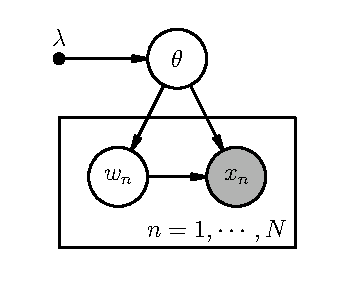
\includegraphics{abstract.pdf}
\end{center}
\caption{%
\figlabel{abstract}}
\end{figure}

In this \paper, we will focus on the problem of inferring the population
parameters from a noisy incomplete \emph{catalog}.
This catalog is defined as some set of posterior probability
functions---preferably represented as samples---for some ``observable'' set of
systems.

\section{The model}

\paragraph{Selection function}
We assume that the selection function is specified by a probability
distribution function that gives the probability of observing a transit with a
given signal-to-noise ratio.
Although we don't perform the integral explicitly, this assumption requires a
marginalization over the period and inclination distribution.
Instead, we choose to model the selection function as a scaled logistic
function of signal-to-noise \sn:
\begin{eqnarray}
p(\isobs=1\,|\,\sn,\,\selection) &=&
\frac{\Pmax}{1+\exp \left [ -(\sn-\snmin) / \selectwidth^2 \right ]} \quad.
\end{eqnarray}
Particular period and inclination distributions imply different values for
\Pmax.

\begin{figure}[htbp]
\begin{center}
    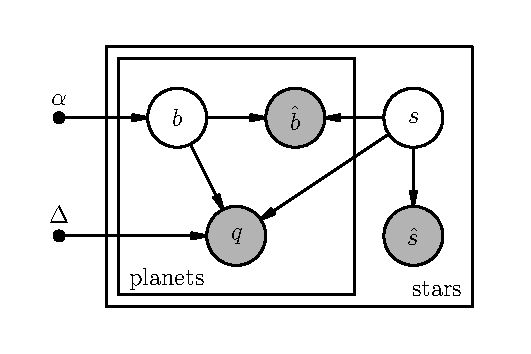
\includegraphics{gm.pdf}
\end{center}
\caption{%
\figlabel{gm}}
\end{figure}

% \begin{deluxetable}{ccl}
% \tablecaption{%
% A description of the model parameters.
% \tablabel{parameters}}
% \tablewidth{0pt}
% \tablehead{& & \colhead{Description}}
% \startdata
% \multirow{3}{*}{\population}
% & $\population_\period$ & The period distribution \\
% & $\population_\radius$ & The exoplanet radius distribution \\
% & $\population_\relincl$ & The relative inclination distribution \\
% \hline
% \selection & --- & The parameters of the catalog selection function \\
% \hline
% $\isobs_{kn}$ & --- & A flag indicating the presence of exoplanet $k$ orbiting
% star $n$ in the catalog \\
% \hline
% \multirow{3}{*}{$\planet_{kn}$}
% & $\period_{kn}$ & The period of exoplanet $k$ orbiting star $n$ (or null) \\
% & $\radius_{kn}$ & The exoplanet's radius \\
% & $\relincl_{kn}$ & The inclination of this orbit away from the systemic mean \\
% \hline
% \multirow{3}{*}{$\planetobs_{kn}$}
% & $\periodobs_{kn}$ & The observed exoplanet period and uncertainty \\
% & $(\rorobs)_{kn}$ & The observed radius ratio and uncertainty \\
% & $\impactobs_{kn}$ & A constraint on the observed impact parameter \\
% \hline
% \multirow{4}{*}{$\stellar_{n}$}
% & $\smass_{n}$ & The mass of star $n$ \\
% & $\sradius_{n}$ & The radius of star $n$ \\
% & $\snoise_{n}$ & The ``variability'' of star $n$ \\
% & $\incl_{n}$ & The mean inclination of the exoplanets in the system $n$ \\
% \hline
% \multirow{2}{*}{$\stellarobs_{n}$}
% & $\sloggobs_{n}$ & The observed surface gravity (and uncertainty) of star $n$ \\
% & $\snoiseobs_{n}$ & The estimated variability of star $n$ \\
% \enddata
% \end{deluxetable}

\acknowledgments
SAMSI. %
It is a pleasure to thank
    \ldots
for helpful contributions to the ideas and code presented here.
This project was partially supported by the NSF (grant AST-0908357), and NASA
(grant NNX08AJ48G).

\newcommand{\arxiv}[1]{\href{http://arxiv.org/abs/#1}{arXiv:#1}}
\begin{thebibliography}{}\raggedright

\bibitem[Fang \& Margot(2012)]{fang}
Fang, J., \& Margot, J.-L.\ 2012, \apj, 761, 92
\arxiv{1207.5250}

\bibitem[Tremaine \& Dong(2012)]{tremaine}
Tremaine, S., \& Dong, S.\ 2012, \aj, 143, 94
\arxiv{1106.5403}

\end{thebibliography}

\end{document}
